%=================================================================
\section{Introduction}\label{sec-intro}


Emotion detection has attracted great interest 
in the natural language processing (NLP)
in the last few years 
~\citep{DBLP:journals/corr/abs-1804-06137,DBLP:journals/corr/abs-1904-00132}.
In the past decades, 
a multitude of different
models have been devised to 
elucidate the nature of human emotion 
~\citep{Scherer2000}. 
A common distinction at the representational level 
of emotions sets dimensional models apart
from discrete or categorical models 
~\cite{Stevenson2007}.

In the categorical approach, 
emotions are represented as 
specific discrete categories,
often with some emotions considered 
more basic than others. 
Ekman’s (1992) theory 
~\cite{Ekman1992}
of six basic emotions 
(joy, sadness, anger, fear, disgust, and surprise) 
is the most well-known,
but also Plutchik’s wheel of emotions
~\cite{Plutchik1980}
 — in which joy, sadness, anger, fear, disgust,
surprise, trust, and anticipation 
are considered most basic — 
is a common framework
in emotion studies. 
However, 
many other theorists provide basic emotion frameworks,
which can count up to fourteen emotion categories 
~\cite{Izard1971,Roseman1984}.

In dimensional models, 
on the other hand, 
emotions are represented as a point in a
multidimensional space. 
According to 
~\cite{Mehrabian1974}, 
every emotional state can be
described by scores 
on the dimensions valence (unhappiness-happiness),
arousal (calmness-excitement) 
and dominance (submission-dominance), 
known as the VAD-model,
as shown in ~\Cref{fig:vad}.. 
However, 
in later work 
~\cite{Russell1980}
argued that 
the two dimensions valence and arousal ,
as shown in ~\Cref{fig:va}.,
suffice for describing emotional states,
whereas 
~\cite{Fontaine2007}
suggest adding a fourth dimension: 
unpredictability.

In this paper, 
we want to predict  
multiple emotion dimension scores for an input text.
A new machine learning paradigm called 
Label Distribution Learning (LDL) 
~\cite{Geng2016}
was proposed in recently years.
Similarly,
we propose an dimensional emotion distribution learning (DEDL) algorithm.
Different from the previous approaches, 
DEDL assumes that
each sentence contains a mixture of 
dimensional emotions with different intensities. 
We can label each sentence with 
an label distribution vector 
where elements corresponds to 
dimensional emotions and 
the value of each element indicates the intensity of the dimensional emotions. 
We require that each vector element has a value 
between 0 and 1 and they sum up to 1.
Use Dimensional Emotions Distribution Learning
to predict multiple emotion dimension scores for an input text.
Then use the predicted VAD and notational VAD to 
do emotion classification.


\begin{figure}[htbp]
	\begin{minipage}[t]{0.5\linewidth}
		\centering
		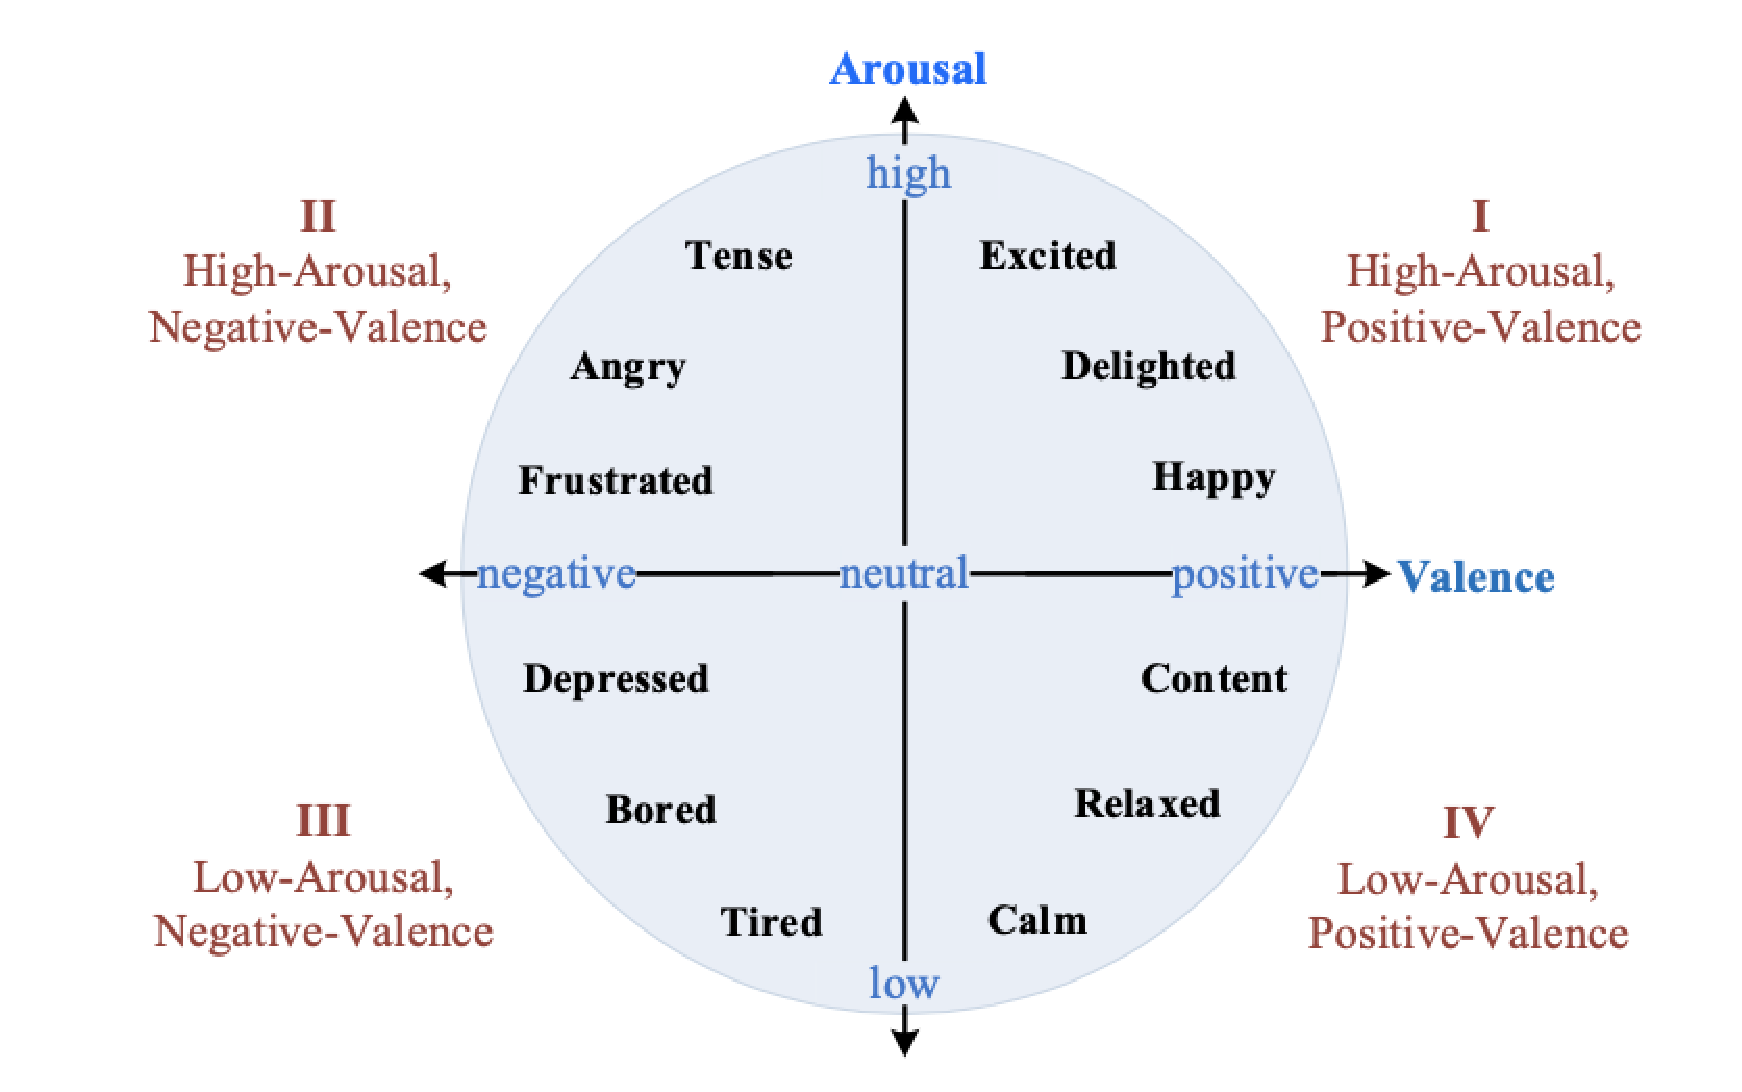
\includegraphics[height=4cm,width=6cm]{figures/va_emotion.eps}
		\caption{The emotional space spanned by the Valence-Arousal model}\label{fig:va}
	\end{minipage}%
	\hfill
	\begin{minipage}[t]{0.5\linewidth}
		\centering
		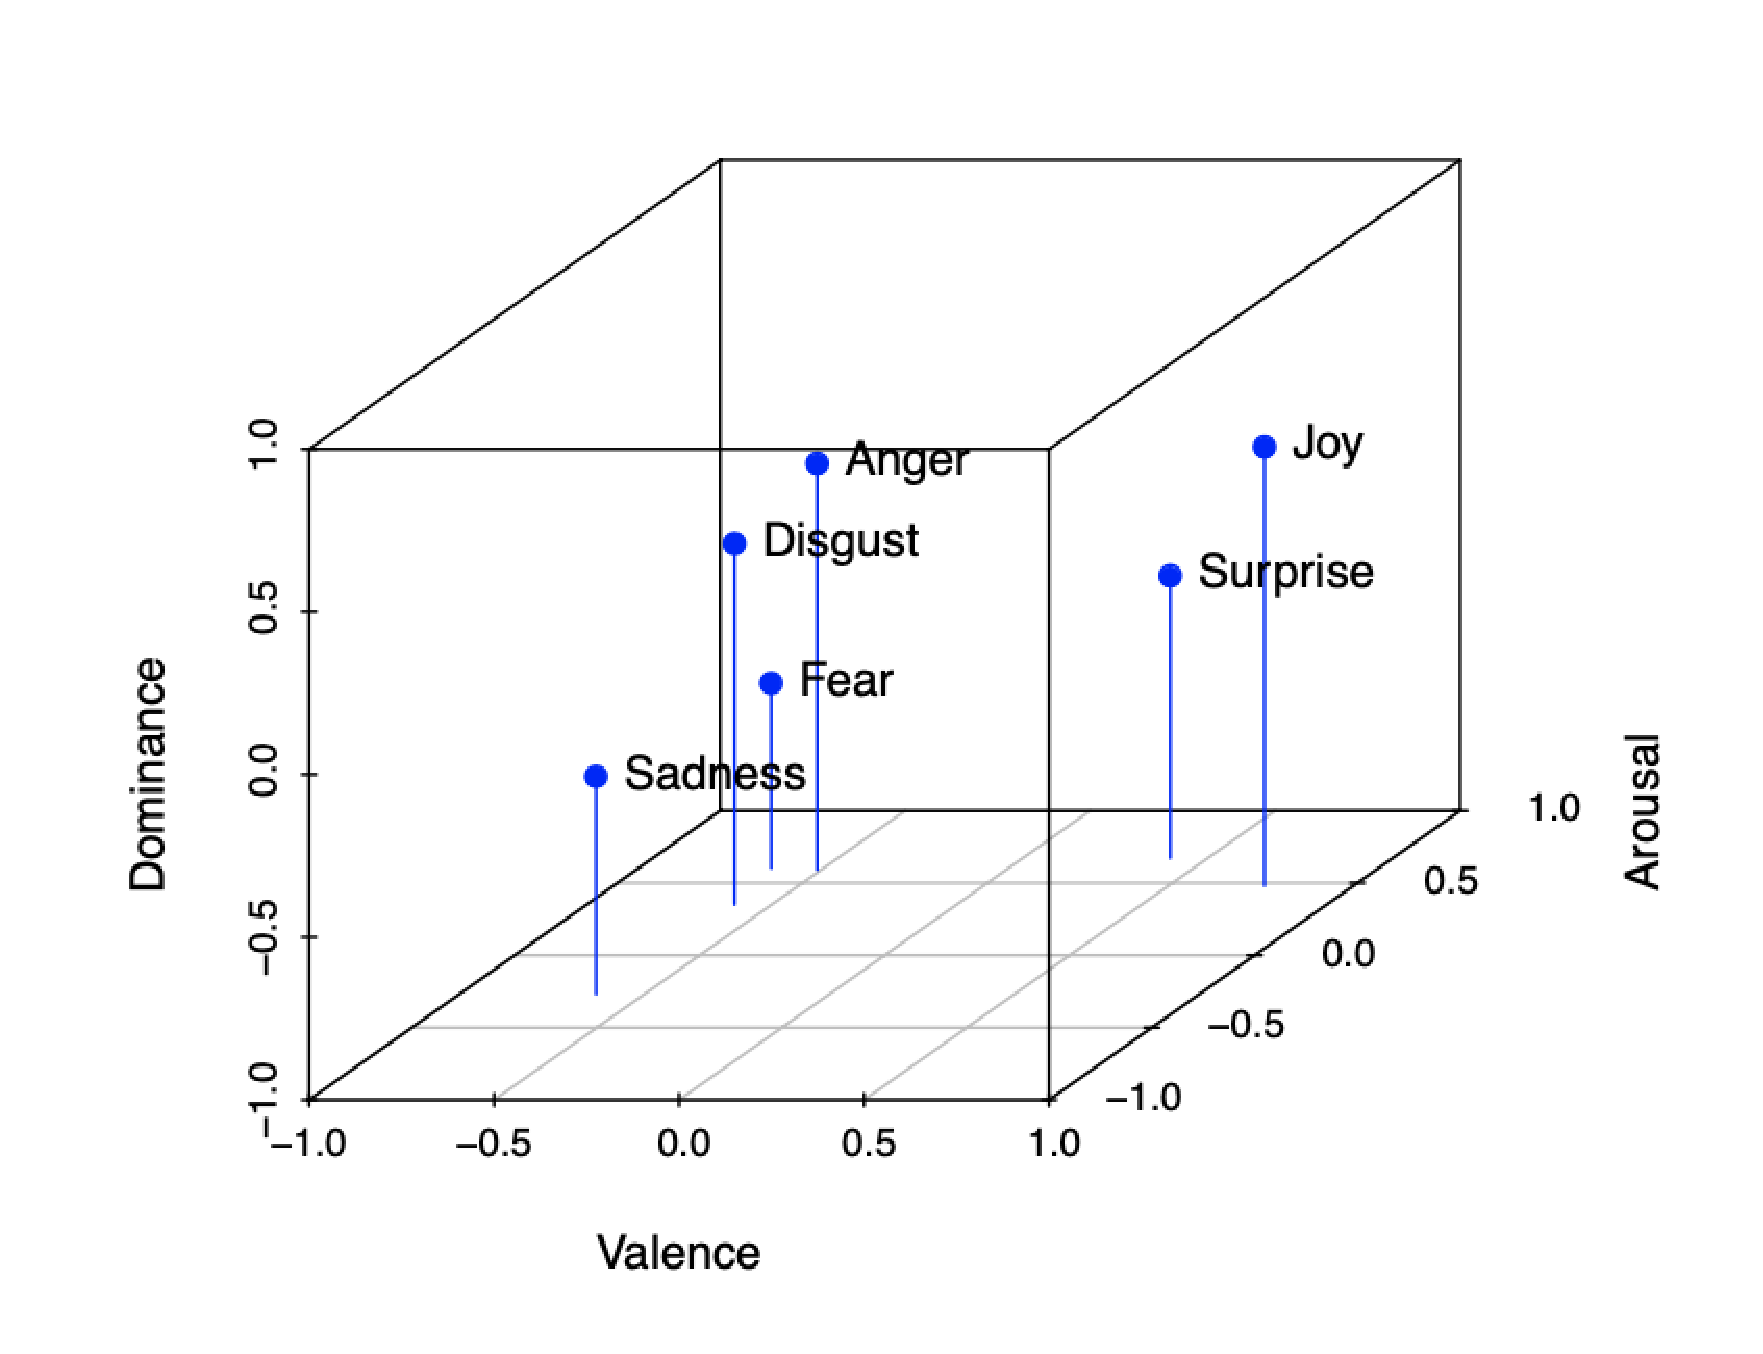
\includegraphics[height=4cm,width=6cm]{figures/six_emotions_vad.eps}
		\caption{The emotional space spanned by the Valence-Arousal-Dominance model. }\label{fig:vad}
	\end{minipage}
\end{figure}

%%==========================================================================================
%%

\section{Preliminary}

For dimensional models, 
a broad variety of stimulus data
bases have been developed, 
predominantly covering lexical stimuli. 
The Affective Norms for English Words (ANEW)
~\cite{Bradley1999}
have been one of the first and
probably most important data sets 
which comprise affective
norms for Valence, Arousal and Dominance
for 1,034 English words. 
In addition, 
larger linguistic units have been considered for 
emotion assessment moving ratings 
from lexical items up to sentence
and text level 
~\cite{Pinheiro2016,}, 
on the one hand, 
and considering alternativemodalities, 
such as pictures and sounds, 
on the other hand 
~\cite{Lang2008,Lang1999}. 
Although these stimulus sets were primarily created
for dimensional representations, 
research activities increasingly
covered discrete emotion representations, 
as well (for all modalities). 
Consequently, 
many of the stimuli which
have formerly been rated according to 
affective dimensions only, 
in the meantime, 
have also received discrete categorical
norm ratings in terms of 
double encodings 
~\cite{Stevenson2008,Stevenson2007}

Due to the severe lack of 
large-scale annotated dimensional emotion distribution corpora,
the predict on dimensional emotion distribution is
later than emotion classification.
~\cite{Yu2015} 
implemented a lexicon- based weighted graph-based approach 
which models the relationship and 
similarity among emotion word nodes 
to rate the Valence-Arousal scores of emotion words. 
Their approach achieved
the better performance over 
the simple linear regression approach, 
the kernel method, and the Pagerank algorithm. 
Preotiuc-Pietro et al. (2016) 
~\cite{Preotiuc-Pietro2016}
collected user information from Facebook, 
and built an English emotion regression corpus 
containing 2,895 texts. 
Wang et al. (2016a) 
~\cite{Jin2016}
proposed a regional CNN-LSTM-based approach 
to document- level emotion regression. 
Their approach first divided a whole text into 
several regions, 
and then extracted regional features 
from each region with multiple CNNs. 
~\cite{Buechel2016}
investigated mapping the dimensional emotion scores to 
an emotion category of a text. 
They first annotated the SemEval07: 
task 14 corpus with dimensional scores, 
and then constructed the mapping 
from dimensional emotion scores to the emotion categories 
by KNN. 
On the basis, 
~\cite{buechel-hahn-2017-emobank}
built an emotion regression corpus, 
namely EMOBANK, 
which contains over 10,000 texts.

Our work is partly inspired by 
~\cite{zhu-etal-2019-adversarial}.
However, our proposed approach differs from 
~\cite{zhu-etal-2019-adversarial}
in two aspects: 
(1) by introducing the
emotion distribution learning framework,
many different criteria can be used to measure the distance
between the true distribution and the predicted distribution,
such as squared $\mathcal{X}^{2}$, Euclidean, Jeffery’s
divergence and Kullback-Leibler divergence
employed in logistic regression model.
(2) the relations between basic emotions are
 captured based on the Plutchik’s wheel of emotions theory to 
 avoid the incorporation of any noisy information 
 from the training data.


%%==========================================================================================
%%

\section{Method} \label{sec-method}

\subsection{Problem Setting}
\

One sentence contain different scores of 
three dimensional emotions. 
We use $ d^y_{x} $ to indicate the intensity of 
dimensional emotion $ y $ for sentence $ x $, 
where $ x \in \chi  $ and $ y \in Y $.
The dimensional emotion intensity is needed to
meet the conditions that
$ d^y_{x} \in [0,1] $ and $\sum_{y}  d^y_{x} = 1$.
Note that $ d^y_{x} $ denotes the proportion that 
$ y $ accounts for in a valence, 
arousal  and dominance dimensional emotion distribution
of $ x $.

And for this problem,
the label distribution set $ D_{i} $ is that
$ D_{i} = \{d^{y_{v}}_{x_{i}},  d^{y_{a}}_{x_{i}}, d^{y_{d}}_{x_{i}}, d^{y_{n}}_{x_{i}}\} $,
where
$ d^{y_{v}}_{x_{i}} = \dfrac{score^{v}_{x_{i}}}{15} $,
$ d^{y_{v}}_{x_{i}} = \dfrac{score^{v}_{x_{i}}}{15} $,
$ d^{y_{v}}_{x_{i}} = \dfrac{score^{v}_{x_{i}}}{15} $,
and $ y_{n} = 1 - y_{v}  - y_{a} - y_{d} $.
The following we proof that 
LDL is valid for the valence, arousal  
and dominance dimensional emotion distribution.


%%==========================================================================================
%%

\subsection{Learning}
\

The training set is $ S = \{ ( x_{i} , D_{i} )  \}^{n}_{i=1} $,
where $ x_{i} \in \chi $ is a sentence embedding and
$ D_{i} = \{d^{y_{1}}_{x_{i}},  d^{y_{2}}_{x_{i}}, ... , d^{y_{c}}_{x_{i}}\} $
is the valence, arousal  and dominance dimensional emotion distribution.

Suppose $ p(y|x) $  is a parametric model
$ p(y|x;{\theta}) $, 
where  $ \theta $ is the parameter vector. 
Given the training set $ S $, 
the goal of DEDL is to find the $ \theta $ that 
can generate a distribution similar to $ D_{i} $
given the instance $ x_{i} $.
As for the Kullback-Leibler divergence,

\begin{equation}\label{eq:kl_divergence}
\theta^{\ast} =
\mathop{\arg\min}\limits_{\theta}
\sum\limits_{i}
\sum\limits_{j}
(d^{y_{j}}_{ x_{ i } }
\ln \dfrac{ d^{y_{j}}_{ x_{ i } } }{ p( y_{ j } | x_{ i } ;{\theta}) })
=\mathop{\arg\max}\limits_{\theta}
\sum\limits_{i}
\sum\limits_{j}
(d^{y_{j}}_{ x_{ i } }
\ln { p( y_{ j } | x_{ i } ;{\theta}) })
\end{equation}

Assumes the parametric model 
$ p(y|x;{\theta}) $ 
to be the maximum entropy model
\cite{BERGER1996},	

\begin{equation}\label{eq:max_entropy}
p(y|x;{\theta}) = \dfrac{1}{Z}
\exp ( \sum\limits_{k}
{\theta}_{y,k} 
g_{k}( \textbf{x})  )
\end{equation}

where $ Z = \sum _{y}
\sum_{k}  {\theta}_{y,k}  g_{k}( \textbf{x}) $
is a normalization factor,
$ {\theta}_{y,k} $ is an element in \textbf {$\theta$} ,
and $ g_{k}( \textbf{x}) $ is the \textit{k}-th feature of\textbf{ x}.
Use a strategy similar to Improved Iterative Scaling (IIS) 
\cite{Della}
to find the best answer.
Substituting ~\Cref{eq:max_entropy} into 
~\Cref{eq:kl_divergence}
yields the target function of $ \theta $

\begin{equation}\label{eq:target_function}
T(\theta) =
\sum\limits_{i,j}
d^{y_{j}}_{ x_{ i } }
\sum\limits_{k}
{\theta}_{y,k} 
g_{k}( \textbf{x})
-
\sum\limits_{i}
\ln\sum\limits_{j}
\exp(\sum\limits_{k}
{\theta}_{y,k} 
g_{k}( \textbf{x}))
\end{equation}

The optimization of 
~\Cref{eq:target_function}
starts with an arbitrary set of parameters.
Then for each step,
it updates the current estimate of
parameters $ \theta +\delta$,
when $\delta$ maximizes a lower bound to
the change in likelihood
$\Omega = T(\theta+\delta) - T(\theta)$.
Then element $\theta_{y_{j},k}$
can be obtained by sloving the equation

\begin{equation}
\sum\limits_{i}
p( y_{ j } | x_{ i } ;{\theta})
g_{k}( \textbf{x})
\exp(
\theta_{y_{j},k}
s(g_{k}(x_{i}))
g^{\#}(x_{i}) )-
\sum\limits_{i}
d^{y_{j}}_{ x_{ i } }
g_{k}(x_{i}) = 0
\end{equation}

where 
$ g^{\#}(x_{i})=\sum\limits_{k}
|g(x_{i})| $
and 
$s(g_{k}(x_{i}) )$
is the sign of 
$g_{k}(x_{i}) $.

%%==========================================================================================
%%

\subsection{Proof}
\

Assume that 

\begin{equation}
T^{\ast}(\theta) =
\mathop{\arg\min}\limits_{\theta}
\sum\limits_{i}
\sum\limits_{j}
(d^{y_{j}}_{ x_{ i } }
\ln \dfrac{ d^{y_{j}}_{ x_{ i } } }{ p( y_{ j } | x_{ i } ;{\theta}) })
\end{equation}

and $ p( y_{ j } | x_{ i } ;{\theta}) $ is the~\Cref{eq:max_entropy}. 
For each step, 
it updates the current estimate of the parameters 
\textbf{$\theta$} to \textbf{ $\theta + \delta$},
where \textbf{$ \delta $} minimizes a lower bound to the change in likelihood

\begin{equation}\label{eq:update}
T^{\ast}(\theta + \delta) - T^{\ast}(\theta) =
\sum\limits_{ij} d^{y_{j}}_{ x_{ i } } ( \ln p(y_{j}|x_{i};{\theta}) - \ln p(y_{j}|x_{i};{\theta +\delta})
\end{equation}

As for the Root Mean Square Error,
the goal is 
$ \mathop{\min}\sum\limits_{ij} ( d^{y_{j}}_{ x_{ i } } -  p(y_{j}|x_{i};{\theta}))^{2}$
which is equal to

\begin{equation}\label{eq:rmse}
	R(\theta) = \mathop{\min} \sum\limits_{ij}
	|d^{y_{j}}_{ x_{ i } } -  p(y_{j}|x_{i};{\theta})|
\end{equation}

for each update,

\begin{equation}\label{eq:rmse'}
	R(\theta + \delta) - R(\theta) \leq 
	\sum\limits_{ij} |
	d^{y_{j}}_{ x_{ i } }  - 
	p(y_{j}|x_{i};{\theta + \delta}) - 
	(d^{y_{j}}_{ x_{ i } }  - 
	p(y_{j}|x_{i};{\theta})) | =
	\sum\limits_{ij}
	|  \ln p(y_{j}|x_{i};{\theta}) - \ln p(y_{j}|x_{i};{\theta +\delta} |
\end{equation}

From the \Cref{eq:update} and \Cref{eq:rmse'}, 
we can find that the goals of EDLD and  RMSE
when the $ \theta $ updates are the same.
So the EDLD is valid.
   

%%==========================================================================================
%%

\section{Experiment and Analysis} \label{sec-experiment}

\subsection{Data Set}
\

Emobank corpus 
\cite{buechel-hahn-2017-emobank}
is composed of 
several categories of 
the Manually Annotated Sub-Corpus of the American National Corpus 
and the corpus of SemEval-2007 Task 14 Affective Text
\cite{Buechel2016}. 
MASC is already annotated on various linguistic levels. 
SE07, on the other hand, bears annotations according to 
Ekman’s six Basic Emotion on a [0,100] scale, respectively. 
This collection of raw data comprises 10,548 sentences see in ~\Cref{tbl:emobank}.

Use the subset MASC corpus to train the DEDL model.
Then use this model to predict the scores of 
Valence, Arousal and Dominance dimensional emotion
for the sentences in the SE07 corpus.
Organize these data into two new data sets:

\begin{description}
	\item [DATA\_1] Predicted VAD is the features and 
	the emotion categories corresponding to 
	the max scales of the sentences in SE07.
	\item [DATA\_2] Annotated VAD is the features and 
	the emotion categories corresponding to 
	the max scales of the sentences in SE07.
\end{description}

\begin{table}[htbp]  \centering
	\caption{Genre distribution of the raw and filtered
		EMOBANK corpus.}
	\label{tbl:emobank}
	\begin{tabular}{cccc}
		\toprule
		Corpus & Domain  & Raw & Filtered  \\
		\midrule
		SE07 &  news headlines &  1250 &  1192 \\
		\hline
		\multirow{6}{*}{MASC} &  blogs&  1378&  1336\\
		&  essays &  1196 &  1135 \\
		&  fiction &  2893 &  2753 \\
		&  letters &  1479 &  1413 \\
		& newspapers & 1381 & 1314 \\
		& traval guides & 971 & 919 \\
		\bottomrule
	\end{tabular}
\end{table}

\subsection{Experiment}

\

\begin{itemize}
	\item
	Data Processing
	
	\begin{itemize}
		\item 
		Use Bert to train the sentence encoding/embedding
		of Emobank corpus, that is the feature vectors $ x_{i} $
		\item 
		Transform the scores of Valence, Arousal and Dominance 
		dimensional emotion into 
		the label distribution 
		$ D_{i} = \{d^{y_{v}}_{x_{i}},  d^{y_{a}}_{x_{i}}, d^{y_{d}}_{x_{i}}, d^{y_{n}}_{x_{i}}\} $,
	\end{itemize}
	
	\item 
	Predict the scores of 
	Valence, Arousal and Dominance dimensional emotion
	through the EDLD
	for the sentences in the SE07 corpus.
	
	\item 
	New Data Set
	
	\begin{itemize}
		\item 
		DATASET\_1 : Predicted VAD is the features and 
		the emotion categories corresponding to 
		the max scales of the sentences in SE07.
		\item 
		DATASET\_2 : Annotated VAD is the features and 
		the emotion categories corresponding to 
		the max scales of the sentences in SE07.
	\end{itemize}
	
	\item 
	Use the following algorithm
	to do emotion calssification.	
	\begin{itemize}
		\item DecisionTree, KNeighbors, LogisticRegression and so on.
		
	\end{itemize}
\end{itemize}

%%==========================================================================================
%%
\subsection{Analysis}
\

For quantitative analysis,
\Cref{tbl:predictedresult}  tabulates the results of the DEDL
on the predictive VAD and the true VAD
by Chebyshev distance (Cheb), 
Clark distance (Clark), Canberra metric (Canber),
 Kullback-Leibler divergence (KL), cosine coefficient (Cosine) 
 and intersection similarity (Intersec).
 
\begin{table} [htbp] \centering
	\caption{The Predicted Results on Six Measures}
	\label{tbl:predictedresult}
	\begin{tabular}{ccccccc}
		\toprule
		Measure & Cheb  & Clark & Canber & KL & Cosine & Intersec\\
		\midrule
		Result &  0.0766 &  0.3521 &  0.4952 & 0.0301 & 0.9912 &0.9234\\
		\bottomrule
	\end{tabular}
\end{table}
 

From the \Cref{tbl:overall-experiments} below
shows the result of emotion classification
on DATA\_1 and DATA\_2.
\cite{Aman2007}
uses the SVC to do emotion classification
among six emotions,
and the accuracy is not much different from
using the VAD.

\begin{table} [htbp] \centering
  \caption{The accuracy of the emotion classification}
  \label{tbl:overall-experiments}
\begin{tabular}{cccccc}
\toprule
 & RandomForest  & Bagging & Boosting & KNN & SVC\\
\midrule
DATA\_1&  0.62 &  0.60 &  0.61 & 0.61 & 0.63\\
DATA\_2 &  0.65 &  0.64 &  0.64 & 0.60 & 0.64\\
\bottomrule
\end{tabular}
\end{table}



%%==========================================================================================
%%\left( 

\section{Conclusions} \label{sec-conclusions}
\
	
	There is not much difference between 
	the values of Valence, Arousal and Dominance 
	dimensional emotions scores predicted by EDLD
	and the labeled VAD.
	But the result of
	emotion classification
	by using traditional machine learning algorithms
	is not very good.
	May we can find the relation between 
	the topological structure of the
    VAD space and the categorical emotion.
	
